Discretization information for DISV grids is read from the file that is specified by ``DISV6'' as the file type.  Only one discretization input file (DISV6, DISU6 or DIS6) can be specified for a model.

The approach for numbering cell and cell vertices for the DISV Package is shown in figure~\ref{fig:gwf-fig3-2}.  The list of vertices for a cell must be in clockwise order.  Closing of the cell polygon by repeating the first vertex as the last vertex is not required in the present implementation.  Internally within the program, however, the first vertex number is added to the end of the vertex list in order to close the polygon.  Thus, users have the option for whether or not to close cell polygons.

\begin{figure}[ht]
	\centering
	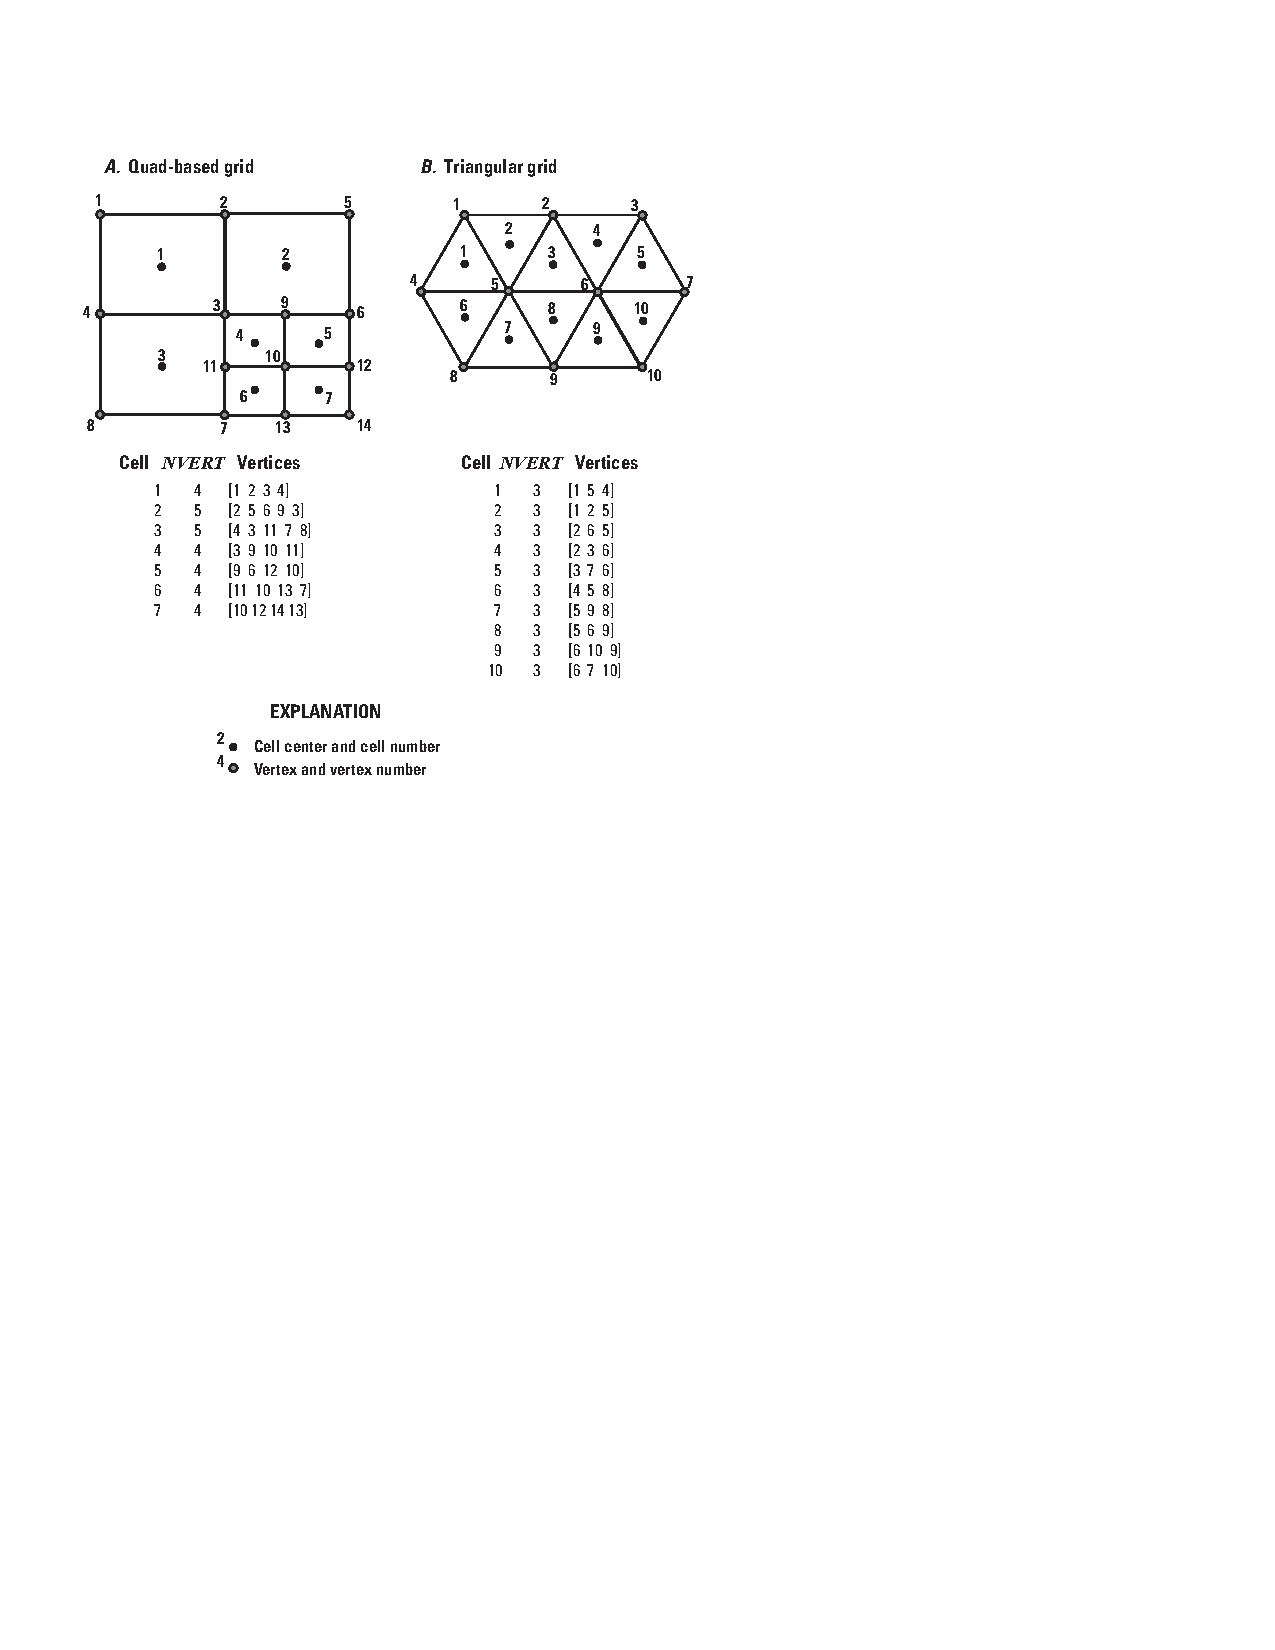
\includegraphics[scale=1.0]{gwf-fig3-2}
	\caption{Schematic diagram showing the vertices and cells defined using the Discretization by Vertices Package. The list of vertices used to define each cell must be in clockwise order.  From \cite{modflow6gwf}}
	\label{fig:gwf-fig3-2}
\end{figure}


\vspace{5mm}
\subsubsection{Structure of Blocks}
\lstinputlisting[style=blockdefinition]{./mf6ivar/tex/gwf-disv-options.dat}
\lstinputlisting[style=blockdefinition]{./mf6ivar/tex/gwf-disv-dimensions.dat}
\lstinputlisting[style=blockdefinition]{./mf6ivar/tex/gwf-disv-griddata.dat}
\lstinputlisting[style=blockdefinition]{./mf6ivar/tex/gwf-disv-vertices.dat}
\lstinputlisting[style=blockdefinition]{./mf6ivar/tex/gwf-disv-cell2d.dat}

\vspace{5mm}
\subsubsection{Explanation of Variables}
\begin{description}
% DO NOT MODIFY THIS FILE DIRECTLY.  IT IS CREATED BY mf6ivar.py 

\item \textbf{Block: OPTIONS}

\begin{description}
\item \texttt{length\_units}---is the length units used for this model.  Values can be ``FEET'', ``METERS'', or ``CENTIMETERS''.  If not specified, the default is ``UNKNOWN''.

\item \texttt{NOGRB}---keyword to deactivate writing of the binary grid file.

\item \texttt{xorigin}---x-position of the origin used for model grid vertices.  This value should be provided in a real-world coordinate system.  A default value of zero is assigned if not specified.  The value for \texttt{xorigin} does not affect the model simulation, but it is written to the binary grid file so that postprocessors can locate the grid in space.

\item \texttt{yorigin}---y-position of the origin used for model grid vertices.  This value should be provided in a real-world coordinate system.  If not specified, then a default value equal to zero is used.  The value for \texttt{yorigin} does not affect the model simulation, but it is written to the binary grid file so that postprocessors can locate the grid in space.

\item \texttt{angrot}---counter-clockwise rotation angle (in degrees) of the model grid coordinate system relative to a real-world coordinate system.  If not specified, then a default value of 0.0 is assigned.  The value for \texttt{angrot} does not affect the model simulation, but it is written to the binary grid file so that postprocessors can locate the grid in space.

\end{description}
\item \textbf{Block: DIMENSIONS}

\begin{description}
\item \texttt{nlay}---is the number of layers in the model grid.

\item \texttt{ncpl}---is the number of cells per layer.  This is a constant value for the grid and it applies to all layers.

\item \texttt{nvert}---is the total number of (x, y) vertex pairs used to characterize the horizontal configuration of the model grid.

\end{description}
\item \textbf{Block: GRIDDATA}

\begin{description}
\item \texttt{top}---is the top elevation for each cell in the top model layer.

\item \texttt{botm}---is the bottom elevation for each cell.

\item \texttt{idomain}---is an optional array that characterizes the existence status of a cell.  If the \texttt{idomain} array is not specified, then all model cells exist within the solution.  If the \texttt{idomain} value for a cell is 0, the cell does not exist in the simulation.  Input and output values will be read and written for the cell, but internal to the program, the cell is excluded from the solution.  If the \texttt{idomain} value for a cell is 1, the cell exists in the simulation.  If the \texttt{idomain} value for a cell is -1, the cell does not exist in the simulation.  Furthermore, the first existing cell above will be connected to the first existing cell below.  This type of cell is referred to as a ``vertical pass through'' cell.

\end{description}
\item \textbf{Block: VERTICES}

\begin{description}
\item \texttt{iv}---is the vertex number.  Records in the VERTICES block must be listed in consecutive order from 1 to \texttt{nvert}.

\item \texttt{xv}---is the x-coordinate for the vertex.

\item \texttt{yv}---is the y-coordinate for the vertex.

\end{description}
\item \textbf{Block: CELL2D}

\begin{description}
\item \texttt{icell2d}---is the cell2d number.  Records in the CELL2D block must be listed in consecutive order from 1 to \texttt{ncpl}.

\item \texttt{xc}---is the x-coordinate for the cell center.

\item \texttt{yc}---is the y-coordinate for the cell center.

\item \texttt{ncvert}---is the number of vertices required to define the cell.  There may be a different number of vertices for each cell.

\item \texttt{icvert}---is an array of integer values containing vertex numbers (in the VERTICES block) used to define the cell.  Vertices must be listed in clockwise order.  Cells that are connected must share vertices.

\end{description}


\end{description}

\vspace{5mm}
\subsubsection{Example Input File}
\lstinputlisting[style=inputfile]{./mf6ivar/examples/gwf-disv-example.dat}
